\documentclass{beamer}
%Information to be included in the title page:
\title{Your Title}
\author{Your Name}
%\institute{Overleaf}
\date{\today}

\begin{document}

%This will make the title slide
\frame{\titlepage}

%Slide 2
\begin{frame}
\frametitle{Slide Title goes here.}
This is some text in the second slide. This is some text in the second slide. This is some text in the second slide.
\end{frame}

%Slide 3
\begin{frame}
\frametitle{A picture}
\begin{center}
\vfill
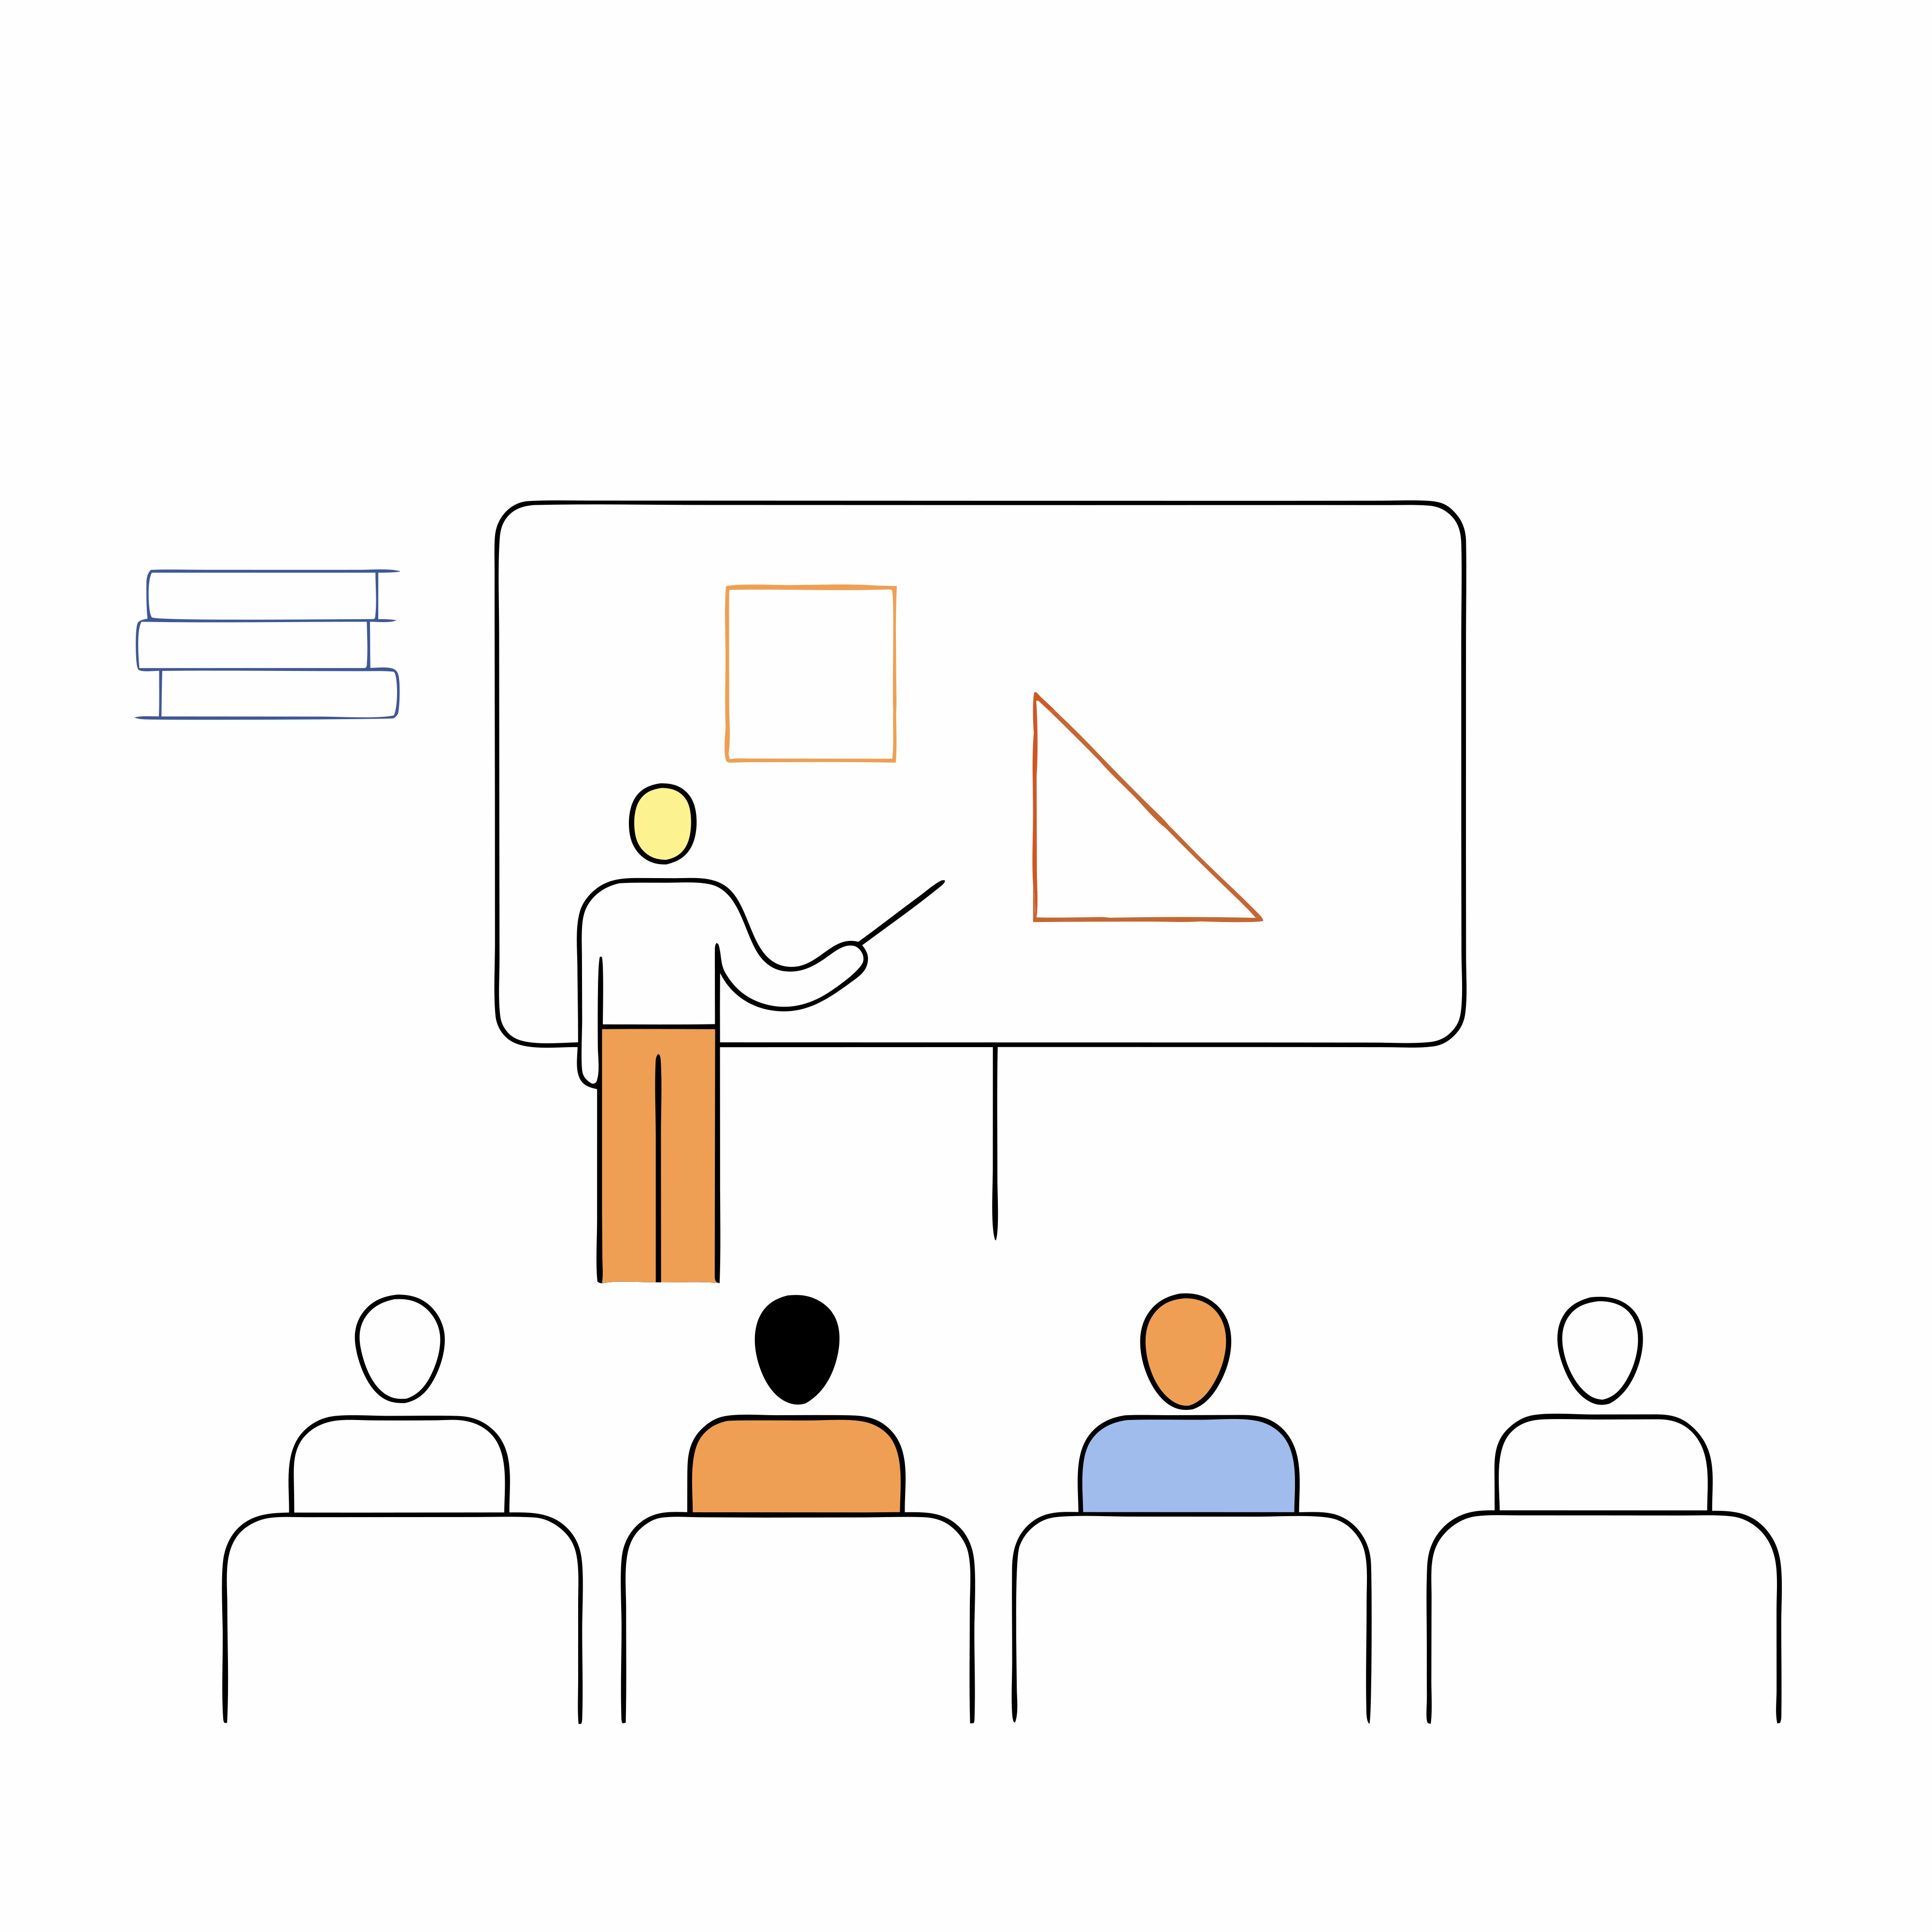
\includegraphics[scale=0.03]{momo.png}
\vfill
\end{center}
\end{frame}

%Slide 4
\begin{frame}
\frametitle{An aligned equation}
\begin{align*}
E &= \sum (y_i - a - bx_i)^2 \\
&= \sum (y_i^2 + a^2 + b^2 x_i^2 - 2ay_i - 2bx_iy_i + 2abx_i) \\
&= \sum y_i^2 + \sum a^2 + \sum b^2 x_i^2 
 - \sum 2ay_i - \sum 2bx_iy_i + \sum 2abx_i \\
&= 1 + na^2 + b^2 - 2br \\
&= (1-r^2) + na^2 + (b - r)^2\ .
\end{align*}
\end{frame}

%Slide 4
\begin{frame}
\frametitle{A list}
\begin{itemize}
\item Do the first step
\item Do the second step
\item Do the third step
\end{itemize}
\end{frame}

%Slide 
\begin{frame}
\frametitle{The Last Slide}
\begin{center}
{\Huge\textcolor{red}{Thank you !!}}
\end{center}
\end{frame}

\end{document}